\documentclass[12pt]{article}
\usepackage[paper=letterpaper,margin=2cm]{geometry}

\usepackage{mathtools, amssymb, amsthm}
\usepackage{graphicx}
\usepackage{tabularx}
\usepackage{titling}
\usepackage{pgfplots}
\usepackage{float}
\usepackage{enumerate}
%%\usepackage[table,xcdraw]{xcolor}
\usepackage{fancyhdr}
\usepackage{polynom}
\usepackage{caption, booktabs}
\usepackage{makecell}
%%\usepackage{cellspace}
%%\setlength\cellspacetoplimit{5pt}
%%\setlength\cellspacebottomlimit{5pt}
\pagestyle{fancy}
\fancyhf{}
\rhead{\small {© 2022 All Rights Reserved, Aiden Rosenberg}}
\rfoot{Page \thepage}

\setlength{\droptitle}{-6em}

\title{AP Classroom Problems}
\author{Aiden Rosenberg}
\date{October 25, 2022 A.D }

\begin{document}
\maketitle
\section*{3.01}
\begin{enumerate}
    \item 
    \begin{center}
        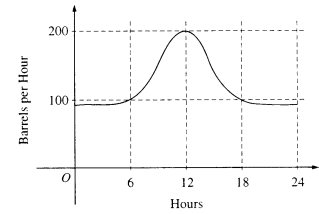
\includegraphics[]{original-7.png}
    \end{center}
    The flow of oil, in barrels per hour, through a pipeline on July 9 is given by the graph shown above. Of the following, which best approximates the total number of barrels of oil that passed through the pipeline that day?
$$\boxed{\int_{0}^{24} B(t) \, dt \approx 3,000}$$
\item 

\begin{table}[H]
\centering
\begin{tabular}{|l||l|l|l|l|}
\hline
$t$ (hours) & 4 & 7 & 12 & 15 \\ \hline
\begin{tabular}[c]{@{}l@{}}$R(t)$\\ (liters per hour)\end{tabular} & 6.5 & 6.2 & 5.9 & 5.6 \\ \hline
\end{tabular}
\end{table}
A tank contains 50 liters of oil at time $t=4$ hours. Oil is being pumped into the tank at a rate $R(t)$ where $R(t)$ is measured in liters per hour, and $t$ is measured in hours. Selected values of $R(t)$ are given in the table above. Using a right Riemann sum with three subintervals and data from the table, what is the approximation of the number of liters of oil that are in the tank at time $t=15$ hours?
$$\int_{4}^{15} R(t) \, dt + R(0)  $$
$$ \approx \biggr((7-4) \cdot R(7) + (12-7) \cdot R(12) +(15-12)\cdot R(17) \biggr) + 50$$
$$=64.9+50$$
$$=\boxed{114.9 \text{ liters}}$$
\item 
\begin{center}
        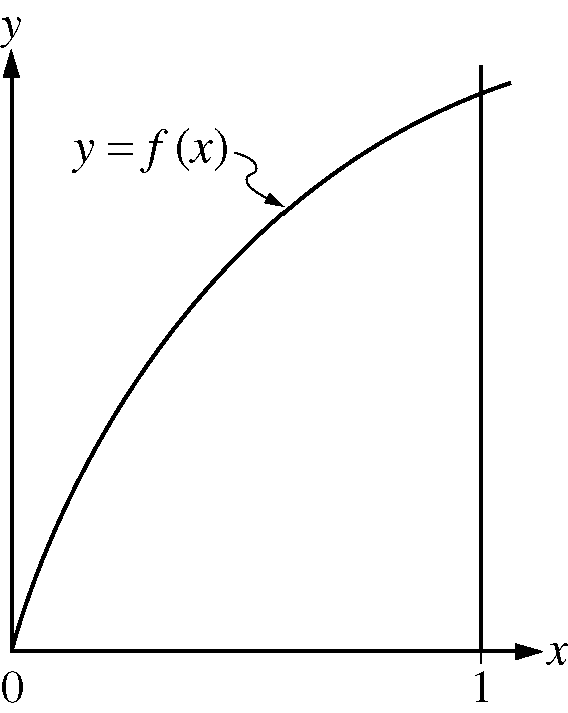
\includegraphics[width=1.5in]{original-8.png}
    \end{center}
A left Riemann sum, a right Riemann sum, and a trapezoidal sum are used to approximate the value of $\int_{0}^{1} f(x) \, dx$, each using the same number of sub intervals. The graph of the function $f$ is shown in the figure above. Which of the sums give an underestimate of the value of $\int_{0}^{1} f(x) \, dx$?
\begin{enumerate}
    \item When $f(x)$ is concave down both left and trapezoidal sums are underestimates. 
\end{enumerate}

$$\boxed{\text{I and III only}}$$
\item 
Let $f$ be the function given by $f(x)=9^x$. If four subintervals of equal length are used, what is the value of the right Riemann sum approximation for $\int_{0}^{2} f(x) \,dx$?
\begin{enumerate}
    \item $\Delta x = 0.5$
\end{enumerate}
$$\text{RHS}_4 = 0.5 \cdot \big( A(0.5) +A(1) +A(1.5)+ A(2) \big)$$
$$\text{RHS}_4 = 0.5 \cdot \big( 3 +9 + 27+ 81 \big)$$
$$\text{RHS}_4 = 0.5 \cdot \big(120)$$
$$\boxed{\text{RHS}_4 = 60}$$
\item 
\begin{table}[H]
\centering
\begin{tabular}{|l||l|l|l|l|l|l|l|}
\hline
$x$ & 0 & 0.5 & 1 & 1.5 & 2 & 2.5 & 3 \\ \hline
$f(x)$ & 0 & 4 & 10 & 18 & 28 & 40 & 54 \\ \hline
\end{tabular}
\end{table}
The table above gives selected values for a continuous function $f$. If $f$ is increasing over the closed interval $[0,3]$, which of the following could be the value of $\int_{0}^{3} f(x)\, dx$?
\begin{enumerate}
\item LHS$_6= 0.5 \big( 0+4+10+18+28+40 \big) = 50$
  \item  RHS$_6= 0.5 \big( 4+10+18+28+40+54 \big) = 77$
\end{enumerate}
$$\text{LHS}_6<\int_{0}^{3} f(x)\, dx <\text{ RHS}_6 $$
$$50<\int_{0}^{3} f(x)\, dx <77 $$
$$\boxed{62 \textit{ Satisfies the necessary conditions}}$$

\item 
\begin{table}[H]
\centering
\begin{tabular}{|l||l|l|l|l|l|l|l|}
\hline
$x$ & 2 & 3 & 5 & 8 & 13 \\ \hline
$f(x)$ & 6 & -2 & -1 & 3 & 9 \\ \hline
\end{tabular}
\end{table}
The function $f$ is continuous on the closed interval $[2,13]$ and has values as shown in the table above. Using the intervals $[2,3]$ , $[3,5]$ , $[5,8]$ , and $[8,13]$ what is the approximation of $\int_{2}^{13} f(x)\, dx$ obtained from a left Riemann sum?

$$\text{LHS}_4 = f(2) \cdot (1) + f(3)\cdot (2) + f(5) \cdot (3) +f(8) \cdot (5)$$
$$\text{LHS}_4 = 6  + (-2)\cdot (2) + (-1) \cdot (3) +(3) \cdot (5)$$
$$\boxed{\text{LHS}_4 = 14}$$

\item 

\begin{table}[H]
\centering
\begin{tabular}{|l||l|l|l|l|l|l|l|}
\hline
$x$ & 0 & $a^2$ & $3a$ & $6a$ & $7a$ \\ \hline
$f(x)$ & 1 & -1 & -3 & -7 & -9 \\ \hline
\end{tabular}
\end{table}
The continuous function $f$ is decreasing for all $x$. Selected values of $f$ are given in the table above, where $a$ is a constant with $0<a<3$. Let $R$ be the right Riemann sum approximation for $\int_{0}^{7a} f(x) \, dx$ using the four subintervals indicated by the data in the table. Which of the following statements is true?
\begin{enumerate}
    \item $$\boxed{R=(a^2-0) \cdot (-1) +(3a-a^2) \cdot (-3) +(6a-3a) \cdot(-7) +(7a-6a) \cdot (-9)}$$ 
    \item $$\boxed{\text{$R$ is an underestimate for } \int_{0}^{7a} f(x) \, dx}$$
\end{enumerate}


\item 
Which of the following is the midpoint Riemann sum approximation of $\int_{4}^{6} \sqrt{x^3+1} \, dx$ using 4 subintervals of equal width?
\begin{enumerate}
    \item $\Delta x = \frac{b-a}{n}= \frac{6-4}{4}=\frac{1}{2}$
    \item $f(x)=\sqrt{x^3+1}$
\end{enumerate}
$$\text{MRAM}_4 = \frac{1}{2} \big( f(4.25) + f(4.75)+ f(5.25)+ f(5.75) \big)$$
$$\boxed{\text{MRAM}_4 = \frac{1}{2} \biggr( \sqrt{4.25^3+1} + \sqrt{4.75^3+1} + \sqrt{5.25^3+1} + \sqrt{5.75^3+1} \biggr)}$$
\newpage
\item 
\begin{table}[H]
\centering
\begin{tabular}{|l||l|l|l|l|l|l|l|}
\hline
$x$ & 0 & 25 & 30 & 50 \\ \hline
$f(x)$ & 4 & 6 & 8 & 12 \\ \hline
\end{tabular}
\end{table}
The values of a continuous function $f$ for selected values of $x$ are given in the table above. What is the value of the left Riemann sum approximation to $\int_{0}^{5} f(x) \,dx$ using the subintervals $[0, 25]$ $[25, 30]$ and $[30, 50]$?

$$\text{LHS}_3 = f(0) \cdot (25) + f(25)\cdot (5) + f(30) \cdot (20) $$
$$\text{LHS}_3 = 4 \cdot (25) + 6 \cdot (5) + 8 \cdot (20) $$
$$\boxed{\text{LHS}_4 = 290}$$
\item 
\begin{table}[H]
\centering
\begin{tabular}{|l||l|l|l|l|l|l|l|}
\hline
$x$ & 0 & 1 & 2 & 3 & 4 & 5 & 6 \\ \hline
$f(x)$ & 0 & 5 & 2 & -1 & -2 & 0 & 3 \\ \hline
\end{tabular}
\end{table}
The function $f$ is continuous on the closed interval $[0, 6]$ and has values as shown in the table above. Using the intervals $[0,2]$, $[2,4]$, and $[4,6]$, what is the approximation of $\int_{0}^{6} f(x) \, dx$ obtained from a midpoint Riemann sum?
$$\text{MRAM}_3 = 2 \big( f(1) + f(3)+ f(5) \big)$$
$$\text{MRAM}_3 = 2 \big( 5 +(-1)+0 \big)$$
$$\boxed{\text{MRAM}_3 = 8}$$
\end{enumerate}
\section*{3.02}
\begin{enumerate}
    \item Let $f$ and $g$ be continuous functions such that $\int_{0}^{10} f(x) \, dx =21$, $\int_{0}^{10} \frac{1}{2}g(x) \, dx =8$, and $\int_{3}^{10} (f(x)-g(x)) \, dx=2$. What is the value of $\int_{0}^{3}(f(x)-g(x)) \,dx$?
   
\begin{enumerate}
    \item $$\int_{0}^{10} \frac{1}{2}g(x) \, dx =8 \Longrightarrow \int_{0}^{10} g(x) \, dx =16$$
     \item $$\int_{0}^{10} (f(x)-g(x)) \, dx=  \int_{0}^{10} f(x) \, dx - \int_{0}^{10} g(x) \,dx = 21-16=5$$
\end{enumerate}
    $$\int_{0}^{10} (f(x)-g(x)) = \int_{0}^{3} (f(x)-g(x)) \, dx  + \int_{3}^{10} (f(x)-g(x)) \, dx$$
    $$\Longrightarrow 2 + \int_{0}^{3} (f(x)-g(x)) \, dx = 5$$
    $$\Longrightarrow \boxed{\int_{0}^{3} (f(x)-g(x)) \, dx =3}$$
    
\item Let $f$ and $g$ be continuous functions for $a \leq x \leq b$. If $a<c<b$, $\int_{a}^{b} f(x) \, dx=P$,$\int_{c}^{b} f(x) \, dx=Q$, $\int_{a}^{b} g(x) \, dx=R$, and $\int_{c}^{b} g(x) \, dx=S$, then $\int_{a}^{c} (f(x)-g(x)) \, dx=$
\begin{enumerate}
    \item $\int_{a}^{c} f(x) \, dx =\int_{a}^{b} f(x) \, dx - \int_{c}^{b} f(x) \, dx = P-Q$
     \item $\int_{a}^{c} g(x) \, dx =\int_{a}^{b} g(x) \, dx - \int_{c}^{b} g(x) \, dx = R-S$
\end{enumerate}
$$\int_{a}^{c} (f(x)-g(x)) \, dx= \int_{a}^{c} f(x) \, dx - \int_{a}^{c} g(x) \, dx $$
$$\Longrightarrow \big(P-Q \big) - \big(R-S \big)$$
$$\Longrightarrow \boxed{P-Q-R+S}$$

\item Let $f$ and $g$ be continuous functions such that $\int^{6}_{0} f(x)\,dx=9$,\\ $\int^{6}_{3} f(x)dx=5$, and $\int^{0}_{3} g(x)dx=-7$. What is the value of $\int^{3}_{0}(\frac{1}{2}f(x)-3g(x))dx$?
\begin{enumerate}
    \item $\int_{0}^{6} f(x) \, dx = \int_{0}^{3} f(x) \, dx + \int_{3}^{6} f(x) \, dx \Longrightarrow \int_{0}^{3} f(x) \, dx = 4$
    \item  $\int^{0}_{3} g(x)dx=-7 \Longrightarrow \int^{3}_{0} g(x)dx=7$
\end{enumerate}

$$\frac{1}{2}\int^{3}_{0}f(x) \, dx -3 \int_{0}^{3} g(x))dx = \frac{1}{2} \cdot 4 - 3 \cdot 7 = \boxed{-19}$$

\item 
\begin{center}
    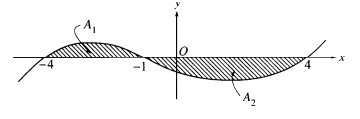
\includegraphics[width=4in]{original-9.png}
\end{center}
The graph of $y=f(x)$ is shown in the figure above. If $A_1$ and $A_2$ are positive numbers that represent the areas of the shaded regions, then in terms of $A_1$ and $A_2$, $\int_{-4}^{4} f(x) \, dx -2 \int_{-1}^{4} f(x) dx=$
\begin{enumerate}
    \item $A_1 = \int_{-4}^{-1} f(x) \, dx$
    \item $A_2 = \int_{-1}^{2} f(x) \, dx$
    \item $A_1-A_2 = \int_{-4}^{4} f(x) \, dx$
\end{enumerate}
$$\int_{-4}^{4} f(x) \, dx -2 \int_{-1}^{4} f(x) dx= (A_1-A_2) - 2(-A_2) = \boxed{A_1+A_2}$$
\newpage
\item Let $f$ and $g$ have continuous first and second derivatives everywhere. If $f(x)\leq g(x)$ for all real $x$, which of the following must be true?
\begin{enumerate}[I.]
    \item $f'(x) \leq g'(x)$ for $x \in \mathbb{R}$ 
    \item $f''(x) \leq g''(x)$ for $x \in \mathbb{R}$
    \item $\int_{0}^{1} f(x) \,dx \leq \int_{0}^{1} g(x) \, dx$
\end{enumerate}
$$\boxed{\text{III only}}$$
\item The function $f$ is defined by $f(x)=\left\{
\begin{array}{ll}
     2 & \text{ for } x <3 \\
      x-1 & \text{ for } x \geq3 \\
\end{array} \right.$ What is the value of $\int_1^5 f(x)\,dx$?
$$\int_{1}^{3} 2 \, dx + \int_{3}^{5} (x-1) \, dx$$
$$2x \biggr\rvert_{1}^{3}  + \biggr[\frac{x^2}{2}-x\biggr]_{3}^{5} = (6-2)+ \biggr(\biggr( \frac{25}{2}-5  \biggr)- \biggr( \frac{9}{2}-3 \biggr)\biggr) = 4+6=\boxed{10}$$


\item 
\begin{center}
    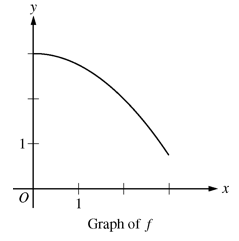
\includegraphics[width=2.5in]{original-10.png}
\end{center}
The graph of the function $f$ is shown above for $0 \leq x \leq 3$. Of the following, which has the least value?
$$\boxed{\text{Right Riemann sum approximation of } \int^3_1 f(x)\,dx \text{ with 4 subintervals of equal length}}$$
\item 
\begin{center}
    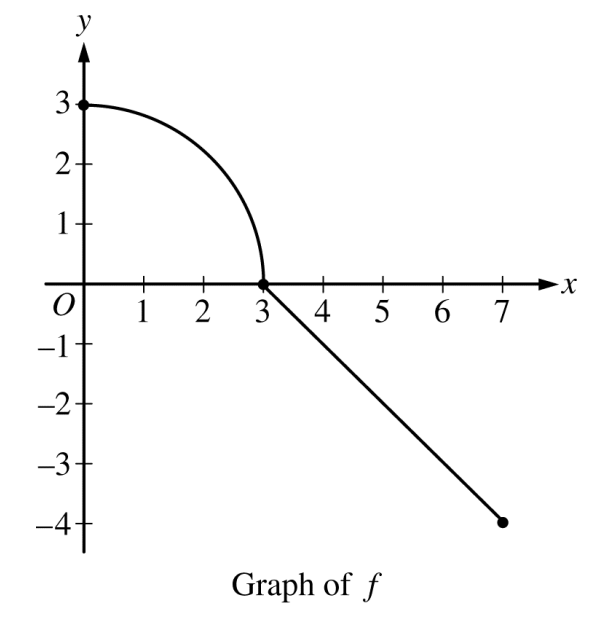
\includegraphics[width=2.5in]{original-11.png}
\end{center}
The graph of the function $f$, which has a domain of $[0, 7]$, is shown in the figure above. The graph consists of a quarter circle of radius 3 and a segment with slope $-1$. Let $b$ be a positive number such that $\int^b_0 f(x)dx=0$.  What is the value of $b$?
\begin{enumerate}
    \item $\int_0^3 f(x) \, dx = \frac{\pi \cdot r^2}{4}= \frac{9\pi}{4}$
    \item $f(x)=\left\{
\begin{array}{ll}
     \sqrt{9-x^2} & \text{ for } x < 3 \\
      3-x & \text{ for } x \geq 3 \\
\end{array} \right.$
\end{enumerate}
$$\int_{3}^{b} (3-x) \, dx = -\frac{9\pi}{4}$$
$$\Longrightarrow  -\frac{9\pi}{4} =3x-\frac{x^2}{2} \biggr\rvert_{3}^{b} = 3b-\frac{b^2}{2}- \big(9-\frac{9}{2} \big)$$
$$\Longrightarrow 12b-2b^2-36+18=-9\pi $$
$$\Longrightarrow 12b-2b^2-18+9\pi=0 \Longrightarrow \boxed{b\approx 6.7599}$$

\item $\int^2_{-1} \frac{|x|}{x}$ is
$$ \int^2_{-1} \frac{|x|}{x} = |x| \biggr\rvert_{-1}^{2} = 2-1=\boxed{1}$$
\item 
\begin{center}
    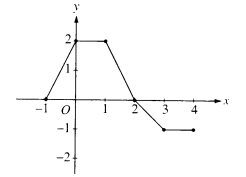
\includegraphics[width=2.5in]{original-12.png}
\end{center}
The graph of a piecewise-linear function $f$, for $-1 \leq x \leq 4$, is shown above. What is the value of $\int_{-1}^{4} f(x) \, dx$?
\begin{enumerate}
    \item $\int_{-1}^{0} f(x) \, dx = (0.5) \cdot (1) \cdot (2) =1$
    \item $\int_{0}^{1} f(x) \, dx = (1) \cdot 2 =2$
    \item $\int_{1}^{2} f(x) \, dx = (0.5) \cdot (1) \cdot (2) =1$
    \item  $\int_{2}^{3} f(x) \, dx = (0.5) \cdot (1) \cdot (-1) =-0.5$
    \item $\int_{3}^{4} f(x) \, dx = (1) \cdot (-1) = -1$
\end{enumerate}
$$\boxed{\int_{-1}^{4} f(x) \, dx =2.5}$$
\end{enumerate}
\section*{3.03}
\begin{enumerate}
    \item If $G(x)$ is an antiderivative for $f(x)$ and $G(2)=-7$, then $G(4)=$
    $$G(4)= G(2) + \int_{2}^{4} f(t) \, dt$$
     $$\boxed{G(4)= -7 + \int_{2}^{4} f(t) \, dt}$$
    \item If the function $f$ is defined by $f(x)=\sqrt{x^3+2}$ and $g$ is an antiderivative of $f$ such that $g(3) = 5$, then $g(1) =$
    $$G(1)=G(3)-\int_{1}^{3} f(x) \,dx$$
    $$\boxed{G(1)\approx -1.585}$$
    \item 
    \begin{center}
        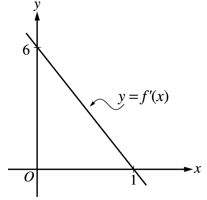
\includegraphics[width=2in]{original-13.png}
    \end{center}
    The graph of $f'$, the derivative of $f$, is the line shown in the figure above. If $f(0)=5$, then $f(1)=$
    $$f(1)=f(0) +\int_0^1 f'(x) \,dx = 5+ (0.1)(6)(3) = \boxed{8}$$
    \item $\int_{0}^{1} \sqrt{x}(x+1) \, dx$

$$\int_{0}^{1} \sqrt{x}(x+1) \, dx = \int_{0}^{1} x^{3/2}+x^{1/2} \, dx$$
$$\Longrightarrow \frac{2x^{5/2}}{5}+ \frac{2x^{2/3}}{3} \biggr\rvert_{0}^{1} = \frac{2}{5}+\frac{2}{3} =\boxed{\frac{16}{15}}$$
    
    \item What are all values of $k$ for which $\int_{-3}^{k} x^2 \,dx=0$
    $$\frac{x^2}{2} \biggr\rvert_{-3}^{k} = \frac{k^3-27}{2}$$
    $$\Longrightarrow \frac{k^3-27}{2} =0 \Longrightarrow \boxed{k=3}$$
    \item $\int_{1}^{2} \frac{x-4}{x^2} \, dx$
$$\int_{1}^{2} \frac{x-4}{x^2} \, dx = \int_{1}^{2} (x^{-1}-4x^{-2}) \, dx = \ln |x| +\frac{4}{x} \biggr\rvert_{1}^{2}= \big( (\ln 2 +2\big) - \big(\ln 1+4 \big) = \boxed{\ln2-2}$$

    
    \item 
    \begin{center}
        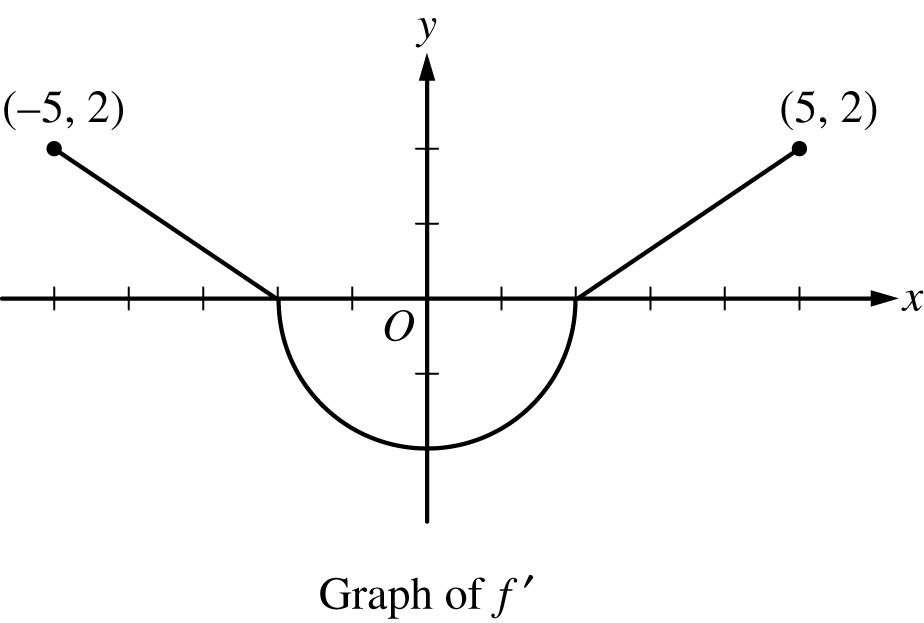
\includegraphics[width=3in]{original-14.png}
    \end{center}
    The graph of $f'$, the derivative of a function $f$, consists of two line segments and a semicircle, as shown in the figure above. If $f(2)=1$, then $f(-5)=$
     \begin{enumerate}
        \item $-\int_{-5}^{2} f'(x) \, dx = \int_{-5}^{-2} f'(x) \, dx + \int_{-2}^{2} f'(x) \, dx$ 
        \item $\int_{-5}^{-2} f'(x) \, dx = (0.5)(3)(2)=3$
        \item $\int_{-2}^{2} f'(x) \, dx = -2\pi$
    \end{enumerate}
    $$f(-5)=f(2)-\int_{-5}^{2} f'(x) \, dx = 1- \big(3 -2\pi \big) = \boxed{2\pi-2}$$
    \item If $n$ is a known positive integer, for what value of $k$ is $\int_{1}^{k} x^{n-1} \,dx = \frac{1}{n}$?
    $$\int_{1}^{k} x^{n-1} \,dx = \frac{x^n}{n} \biggr\rvert_{1}^{k} = \frac{k^n}{n} -\frac{1^n}{n} $$
$$\frac{k^n -1}{n}= \frac{1}{n} \Longrightarrow k^n=2 $$
$$\Longrightarrow \boxed{k= 2^{1/n}}$$

    
    \item If $g(x)=x^2-3x+4$ and $f(x)=g'(x)$, then $\int_{1}^{3} f(x) \, dx =$
    \begin{enumerate}
        \item $g(3)=3^2-3(3)+4=4$
        \item $g(1)=1-3+4=2$
    \end{enumerate}
    $$\int_{1}^{3} f(x) \, dx =\int_{1}^{3} g'(x) \, dx = g(3)-g(1) = 4-2= \boxed{2}$$
    
    \item Let $F(x)$ be an antiderivative of $\frac{(\ln x)^3}{x}$ . If $F(1)=0$, then $F(9)=$
    $$F(9)=F(1) +\int_{1}^{9} \frac{(\ln x)^2}{x} \, dx$$
    $$\boxed{F(9) \approx 5.827}$$
\end{enumerate}
\section*{3.04}
\begin{enumerate}
    \item If $\frac{dy}{dx}=-10e^{-t/2}$ and $y(0)=20$, what is the value of $y(6)$?
$$y(6)=y(0)+ \int_{0}^{6} -10e^{-t/2} \, dt$$
$$y(6)=y(0)+ 20e^{-t/2} \biggr\rvert_{0}^{6}$$
$$y(6)=20+ (20e^{-3}-20) = \boxed{20e^{-3}}$$
    
    
    \item Let $f$ be a differentiable function such that $f(1)=\pi$ and $f'(x)=\sqrt{x^3+6}$. What is the value of $f(5)$?
    $$f(5)=f(1)+\int_{1}^{5} f'(x) \,dx$$
    $$f(5)=\pi + \int_{1}^{5} \sqrt{x^3+6} \, dx$$
    $$\boxed{f(5)\approx 27.814}$$
    \item 
\begin{table}[h]
\centering
\begin{tabular}{|l||l|l|l|l|}
\hline
$x$ & 0 & 1 & 2 & 3 \\ \hline\hline
$f(x)$ & 5 & 2 & 3 & 6 \\ \hline
$f'(x)$ & -3 & 1 & 3 & 4 \\ \hline
\end{tabular}
\end{table}
The derivative of the function $f$ is continuous on the closed interval $[0,4]$. Values of $f$ and $f'$ for selected values of $x$ are given in the table above. If $\int_{0}^{4} f'(t)\, dt=8$, then $f(4) =$
$$\int_{0}^{4} f'(t)\, dt = f(4)-f(0) =8$$
$$f(4)=8+f(0) = \boxed{13}$$

\item $\int_{0}^{x} \sin t \, dt =$
$$\int_{0}^{x} \sin t \, dt = -\cos(t)\biggr\rvert_{0}^{x} = -\cos(x)+\cos (0) = \boxed{1-\cos(x)} $$
\item $\int_1^2 \frac{dx}{2x+1}=$
\begin{enumerate}
    \item Let $u=2x+1 \Longrightarrow du =2dx$
\end{enumerate}
$$\frac{1}{2}\int_{3}^{5} \frac{1}{u} \, du = \frac{\ln u}{2} \biggr\rvert_{3}^{5} = \boxed{\frac{1}{2} (\ln 5 -\ln 3)}$$
\item If $\int_{0}^{k} (2kx-x^2) \, dx = 18$ , then $k=$
$$\int_{0}^{k} (2kx-x^2) \, dx = kx^2-\frac{x^3}{3}\biggr\rvert_{0}^{k} = k^3-\frac{k^3}{3} = \frac{2k^3}{3}$$
$$18= \frac{2k^3}{3} \Longrightarrow 27=k^3$$
$$\boxed{k=3}$$


\item If the function $f$ has a continuous derivative on $[0,c]$, then $\int_{0}^{c} f'(x) \,dx=$
$$\boxed{f(x)-f(0)}$$
\item Let $g$ be a differentiable function such that $g(10)=2e$ and $g'(x)=5e^{-\sqrt{x}}$. What is the value of $g(2)$?
$$g(2)=g(10)-\int_{2}^{10} g'(x) \, dx$$
$$\boxed{g(2)\approx 1.329}$$
\item 
\begin{table}[h]
\centering
\begin{tabular}{|l||l|l|l|l|}
\hline
$x$ & 0 & 1 & 2 & 3 \\ \hline\hline
$f(x)$ & 4 & 9 & 12 & 10 \\ \hline
$f'(x)$ & 5 & 4 & 1 & -6 \\ \hline
\end{tabular}
\end{table}
Selected values of the twice-differentiable function $f$ and its derivative $f'$ are given in the table above. What is the value of $\int_{0}^{3} f'(x) \, dx$?
$$\int_{0}^{3} f'(x) \, dx = f(3)-f(0)=10-4= \boxed{6}$$

\item Let $g$ be a differentiable function such that $g(4)=0.325$ and $g'(x)=\frac{1}{x}e^{-x}(\cos(\frac{x}{100}))$. What is the value of $g(1)$?
$$g(1)=g(4)-\int_{1}^{4}g'(x) \, dx $$
$$\boxed{g(1)\approx 0.109}$$

\item 
\begin{table}[H]
\centering
\begin{tabular}{|l||l|l|l|l|}
\hline
$x$ & 0 & 2 & 4 & 6 \\ \hline\hline
$f(x)$ & -22 & -6 & 2 & 2 \\ \hline
$f'(x)$ & 10 & 6 & 2 & -2 \\ \hline
\end{tabular}
\end{table}
Selected values of the twice-differentiable function $f$ and its derivative $f'$ are given in the table above. What is the value of $\int_{0}^{6} f'(x) \, dx$?
$$\int_{0}^{6} f'(x) \, dx = f(6)-f(0)=2-(-22)= \boxed{24}$$
\item Let $f$ be a continuous function on the closed interval $[0,2]$. If $2\leq f(x)\leq4$, then the greatest possible value of $\int_{0}^{2} f(x) \, dx$ is
$$\int_{0}^{2} 2 \, dx  = 2x\biggr\rvert_{0}^{2}=\boxed{8}$$
\item $\int_{1}^{4} |x-3| \, dx = $
\begin{enumerate}
    \item Let $f(x)=|x-3|$
\end{enumerate}
$$f(x)=\left\{
\begin{array}{ll}
     3-x & \text{ for } x < 3 \\
      x-3 & \text{ for } x \geq 3 \\
\end{array} \right.$$
$$\int_{1}^{4} |x-3| \, dx = \int_{1}^{3} (3-x) \, dx + \int_{3}^{4} (x-3) \, dx $$
$$\int_{1}^{4} |x-3| \, dx = 3x-\frac{x^2}{2} \biggr\rvert_{1}^{3} + \frac{x^2}{2}-3x \biggr\rvert_{3}^{4}  $$
$$\Longrightarrow \biggr((9-4.5)-(3-0.5) \biggr) + \biggr((8-12)-(4.5-9) \biggr) $$
$$\Longrightarrow (2)+(0.5)=\boxed{2.5}$$

\end{enumerate}
\section*{3.05}
\begin{enumerate}
    \item If $0\leq b \leq 2$, for what value of $b$ is $\int_{0}^{b} \cos(e^x) \, dx$ a minimum?
    $$F(x)=\int_{0}^{x} \cos(e^t) \, dt$$
    $$F'(x)=\cos(e^x) $$
  $$F'(x)<0 \text{ when } x\in[0.451,1.550]$$
  $$ F'(x)>0 \text{ when } x\in[0, 0.451] \text{ and when } x\in[1.550,2]$$
  $$\boxed{\text{When } x\approx 1.550 \Longrightarrow F(x) \text{ has a local minimum}}$$
  \newpage
    \item Let $g$ be a function with first derivative given by $g'(x)=\int_{0}^{x} e^{-t^2} \, dt$. Which of the following must be true on the interval $0<x<2$?
    \begin{enumerate}
        \item $g'(x)=\int_{0}^{x} e^{-t^2} \, dt \Longrightarrow g'(x)>0 \text{ when } x\in[0,2] \Longrightarrow g'(x)>0 \text{ when } x\in[0,2]$
        \item $g''(x)=\frac{d}{dx}\biggr(\int_{0}^{x} e^{-t^2}\, dt\biggr)=e^{-x^2} \Longrightarrow g''(x)>0 \text{ when } x\in[0,2]$
        \item Note that $e^{x}>0$ for all $x\in \mathbb{R}$
    \end{enumerate}
    $$\boxed{\text{$g$ is increasing, and the graph of $g$ is concave up.}}$$
    \item 
    \begin{center}
        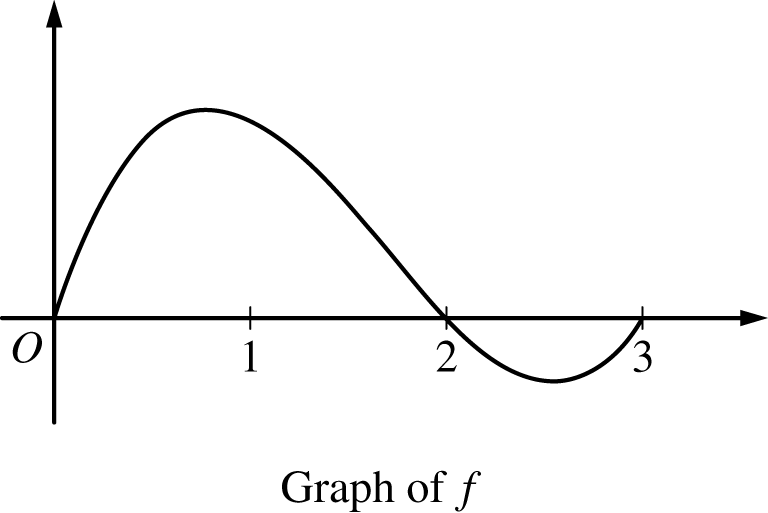
\includegraphics[width=2in]{original-15.png}
    \end{center}
    The graph of the differentiable function $f$ is shown in the figure above. Let $h$ be the function defined by $h(x)=\int^{x}_{0}f(t)\,dt$. Which of the following correctly orders $h(2)$, $h'(2)$, and $h''(2)$?
    \begin{enumerate}
        \item $h(2) = \int^{x}_{2}f(t)\,dt >2$ \textit{Area of the graph}
        \item $h'(2)=0$ \textit{Point of the function}
        \item $h''(2)<0$ \textit{Slope of the tangent line}
    \end{enumerate}
  $$  \boxed{h''(2)<h'(2)<h(2)}$$
    \item 
    \begin{center}
        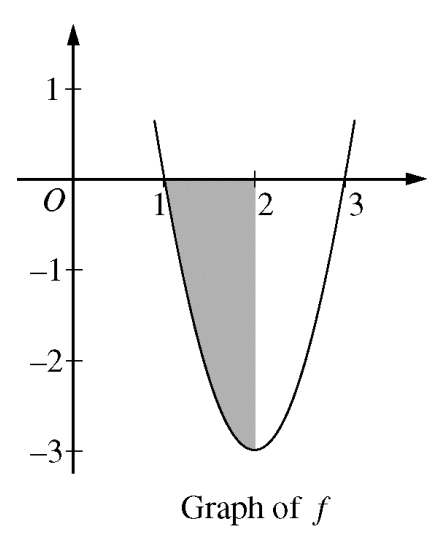
\includegraphics[width=1.5in]{original-16.png}
    \end{center}
    The figure above shows the graph of the function $f$. If $g(x)=\int_{1}^{x}f(t)\,dt$ and the shaded region has an area of $2$, what is the value of $g(2)$?
    $$\boxed{g(2)=\int_{1}^{2}f(t)\,dt=-2}$$
    \newpage
    \item If is the function given by $f(x)=\int_{4}^{2x} \sqrt{t^2-t} \, dt$, then $f'(2)=$
$$F'(x)=\frac{d}{dx}\biggr( \int_{4}^{2x} \sqrt{t^2-t} \, dt \biggr)= \frac{d}{dx}\biggr( F(2x)-f(4) \biggr)$$
    $$F'(x)=2F'(2x)= 2\sqrt{4x^2-2x}$$
$$F'(2)= 2\sqrt{4(2)^2-2(2)}=\boxed{2\sqrt{12}}$$
    
    \item $\frac{d}{dx}\biggr( \int_{0}^{x^2} \sin(t^3) \, dt \biggr)=$
$$F'(x)=\frac{d}{dx}\biggr( \int_{0}^{x^2} \sin(t^3) \, dt \biggr) = \frac{d}{dx}\biggr( F(x^2)-F(4) \biggr)$$
 $$F'(x)=2x \cdot F'(x^3)= \boxed{2x\sin(x^6)}$$

    \item $\frac{d}{dx}\biggr( \int_{0}^{x} \sqrt{1+t^2} \, dt \biggr)=$
$$F(x)=\frac{d}{dx}\biggr( \int_{0}^{x} \sqrt{1+t^2} \, dt \biggr) = \frac{d}{dx}\biggr( F(x)-F(0) \biggr)$$
$$F'(x)=\boxed{\sqrt{1+x^2}}$$

    
    \item If $F(x)=\int_{0}^{x} \sqrt{t^3+1} $, then $F'(2)=$
    $$F'(x)=\frac{d}{dx}\biggr( \int_{0}^{x} \sqrt{t^3+1} \, dt \biggr) = \frac{d}{dx}\biggr( F(x)-F(0) \biggr)$$ 
$$F'(x)=f(x)=\sqrt{x^3+1}$$
$$F'(2)=\sqrt{(2)^3+1}=\boxed{3}$$
\newpage
    \item 
     \begin{center}
        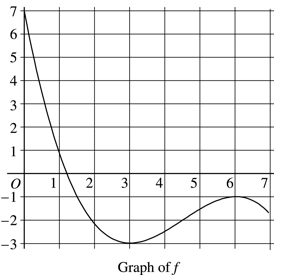
\includegraphics[width=2.5in]{original-17.png}
    \end{center}
    The graph of the function $f$ shown in the figure above has horizontal tangents at $x = 3$ and $x = 6$. If $g(x)=\int_{0}^{2x} f(t) \, dt$ what is the value of $g'(3)$?
    $$g'(x)=\frac{d}{dx}\biggr( \int_{0}^{2x} f(t) \, dt \biggr) = \frac{d}{dx}\biggr( g(2x)-g(0) \biggr)$$ 
    $$g'(x)= 2 \cdot f(2x) = \boxed{-2}$$
    \item 
    \begin{center}
        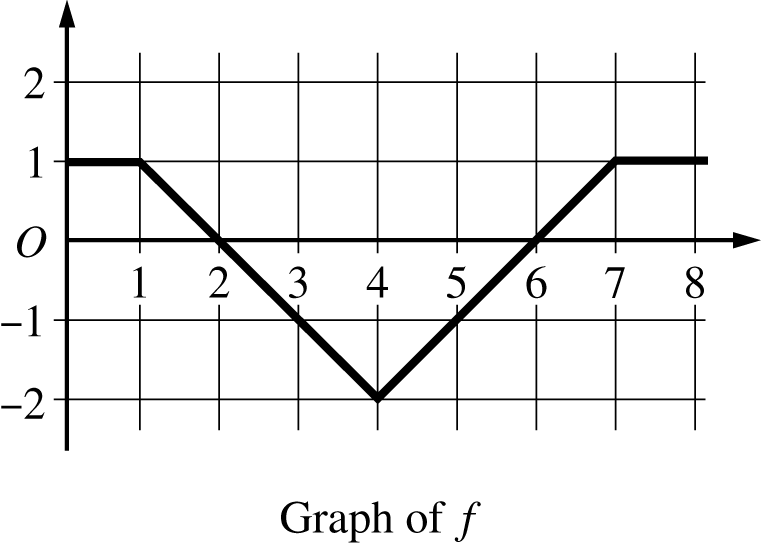
\includegraphics[width=2.5in]{original-18.png}
    \end{center}
    The graph of the function $f$ in the figure above consists of four line segments. Let $g$ be the function defined by $g(x)=\int_{0}^{x} f(t) \, dt$. Which of the following is an equation of the line tangent to the graph of $g$ at $x=5$?
    
    $$g'(x)=\frac{d}{dx}\biggr( \int_{0}^{x} f(t) \, dt \biggr) = \frac{d}{dx}\biggr( g(x)-g(0) \biggr)$$ 
    $$g'(x)= f(x) $$
    \begin{enumerate}
        \item $g'(5)=-1$
        \item $g(5)=\int_0^5 f(t) \, dt = 1.5-3.5=-2$
    \end{enumerate}
    $$y=-1(x-5)-2=\boxed{3-x}$$
\end{enumerate}
\section*{3.06}
\newpage
\begin{enumerate}
    \item Which of the following are equivalent to $\int_{2}^{4}\frac{2x+5}{5-x} \, dx$?
   $$\polylongdiv{2x+5}{5-x}$$
   $$\frac{2x+5}{5-x} = \frac{15}{5-x} -2$$
   $$\Longrightarrow  \int_{2}^{4} \biggr(\frac{15}{5-x} -2 \biggr) \, dx$$
\begin{enumerate}
    \item Let $u=5-x $
    \item $du=-dx$
\end{enumerate}
$$\Longrightarrow -\int_{3}^{1} \biggr(\frac{15}{u} -2 \biggr) \, du $$
$$\Longrightarrow \int_{1}^{3} \biggr(\frac{15}{u} -2 \biggr) \, du = 15\ln(3)-4$$
$$\boxed{\text{II and III only}}$$

   
    \item Which of the following is equivalent to $\int_{3}^{5} x \ln x \, dx$?
\begin{enumerate}
    \item $u=\ln(x) \Longrightarrow du= \frac{1}{x} \, dx$
    \item $dv=x \,dx \Longrightarrow v=\frac{x^2}{2}$
    \item $\int u \, dv = uv- \int v \, du$
\end{enumerate}
$$\boxed{\Longrightarrow \frac{1}{2}x^2\ln(x) \biggr\rvert_{3}^{5} -\int_{3}^{5} \frac{x}{2} \, dx}$$
    
    \item Let $f$ be the function defined by $f(x)=\int_{0}^{x} (2t^3-15t^2+36t) \, dt$. On which of the following intervals is the graph of $y=f(x)$ concave down?
    \begin{enumerate}
        \item $f'(x)=\frac{d}{dx}\big(\int_{0}^{x} (2t^3-15t^2+36t) \, dt \big) = 2x^3-15x^2+36x$
        \item $f''(x)=6x^2-30x+36 = 6(x-2)(x-3)$
    \end{enumerate}
$$\boxed{\text{When } x\in[2,3] \: f''(x)<0 \: \therefore \: f \text{ is concave down.}}$$
\item 
\begin{table}[h]
\centering
\begin{tabular}{|l||l|l|l|l|}
\hline
$x$ & -4 & -3 & -2 & -1 \\ \hline
$f(x)$ & 0.75 & -1.5 & -2.25 & -1.5 \\ \hline
$f'(x)$ & -3 & -1.5 & 0 & 1.5 \\ \hline
\end{tabular}
\end{table}
The table above gives values of a function $f$ and its derivative at selected values of $x$. If $f'$ is continuous on the interval $[-4,-1]$ what is the value of $\int_{-4}^{-1} f'(x) \, dx$?
$$\int_{-4}^{-1} f'(x) \, dx = f(-1)-f(-4) = -1.5-0.75=\boxed{-2.25}$$
\item If $f'(x)=\sin\big(\frac{\pi e^x}{2}\big)$ and $f(0)=1$, then $f(2)=$
$$f(2)=f(0)+\int_{0}^{2}f'(x) \, dx$$
$$f(2)=f(0)+\int_{0}^{2}\sin\biggr(\frac{\pi e^x}{2}\biggr) \, dx$$
$$\boxed{f(2) \approx 1.157}$$
\item
\begin{center}
    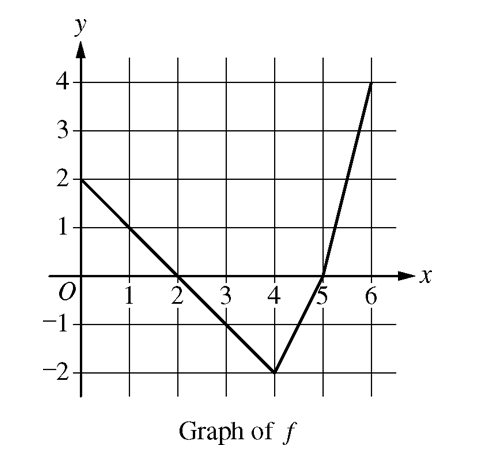
\includegraphics[width=2in]{original-19.png}
\end{center}
The graph of the function $f$, shown above, consists of three line segments. If the function $g$ is an antiderivative of $f$ such that $g(2)=5$, for how many values of $c$, where $0 \leq c \leq 6$, does $g(c) = 3$?
\begin{enumerate}
    \item $g(0)=f(2)-\int_{0}^{2} f(t) \, dt = 5-2=3$
    \item $g(4)=f(2)+\int_{2}^{4} f(t) \, dt = 5+(-2)=3$
    \item $g(5)=f(2)+\int_{2}^{5} f(t) \, dt = 5+(-2)-1=2$
    \item $g(6)=f(2)+\int_{2}^{6} f(t) \, dt = 5+(-3)+2=4$
    \item Since $g$ is continuous for $[5,6]$ and $3\in[f(5),f(6)]$ than there is a $c\in[5,6]$ such that $f(c)=3$
\end{enumerate}
$$\boxed{\text{three}}$$
\item
\begin{center}
    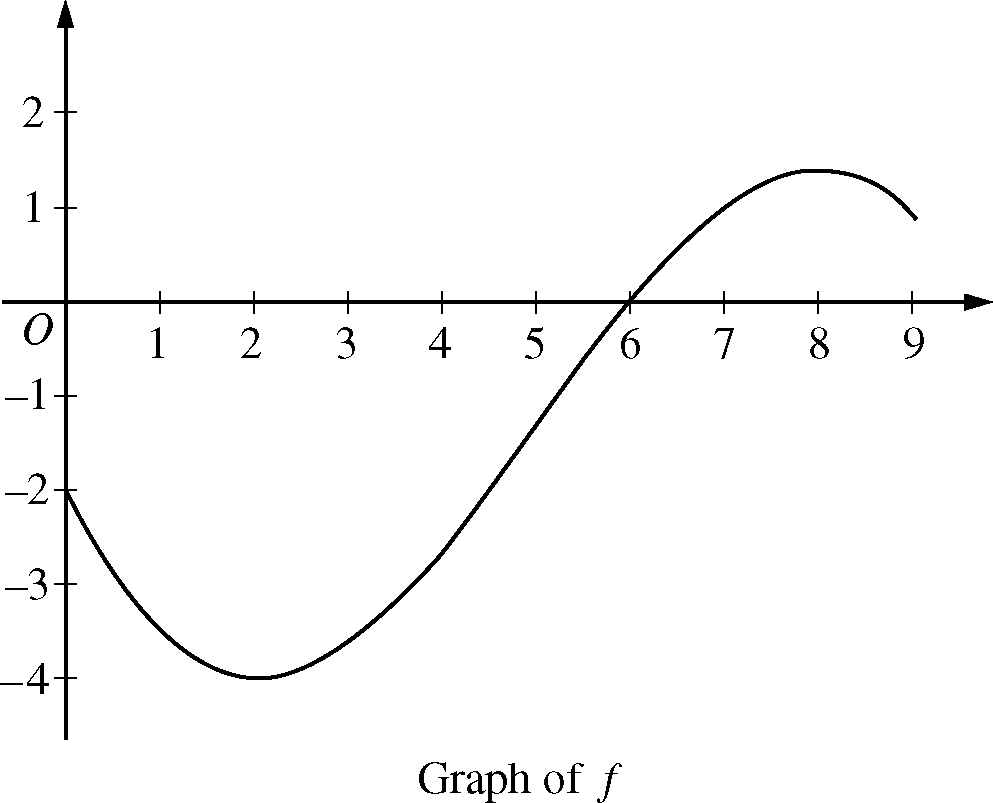
\includegraphics[width=3in]{original-20.png}
\end{center}
The graph of a differentiable function f is shown above. If $h(x)=\int_{0}^{x} f(t) \, dt$, which of the following is true?
\begin{enumerate}
    \item $h(6)= \int_{0}^{6} f(t) \, dt < 0$
    \item $h'(6)= f(6) = 0$
    \item $h''(6)=f'(6)>0$
\end{enumerate}
$$\boxed{h(6)< h'(6)< h''(6)}$$

\item Let $f$ be the function given by $f(x)=\int_{10}^{x} (-t^2+2t+3) \, dt$. On what intervals is $f$ increasing?
\begin{enumerate}
    \item $f'(x)= \frac{d}{dx}\big(\int_{10}^{x} (-t^2+2t+3) \, dt \big)=-x^2+2x+3 =-(x-3)(x+1)$
\end{enumerate}
$$\boxed{\text{When } x\in[-1,3] \: f'(x)>0 \: \therefore \: f \text{ is increasing.}}$$

\item 
\begin{center}
    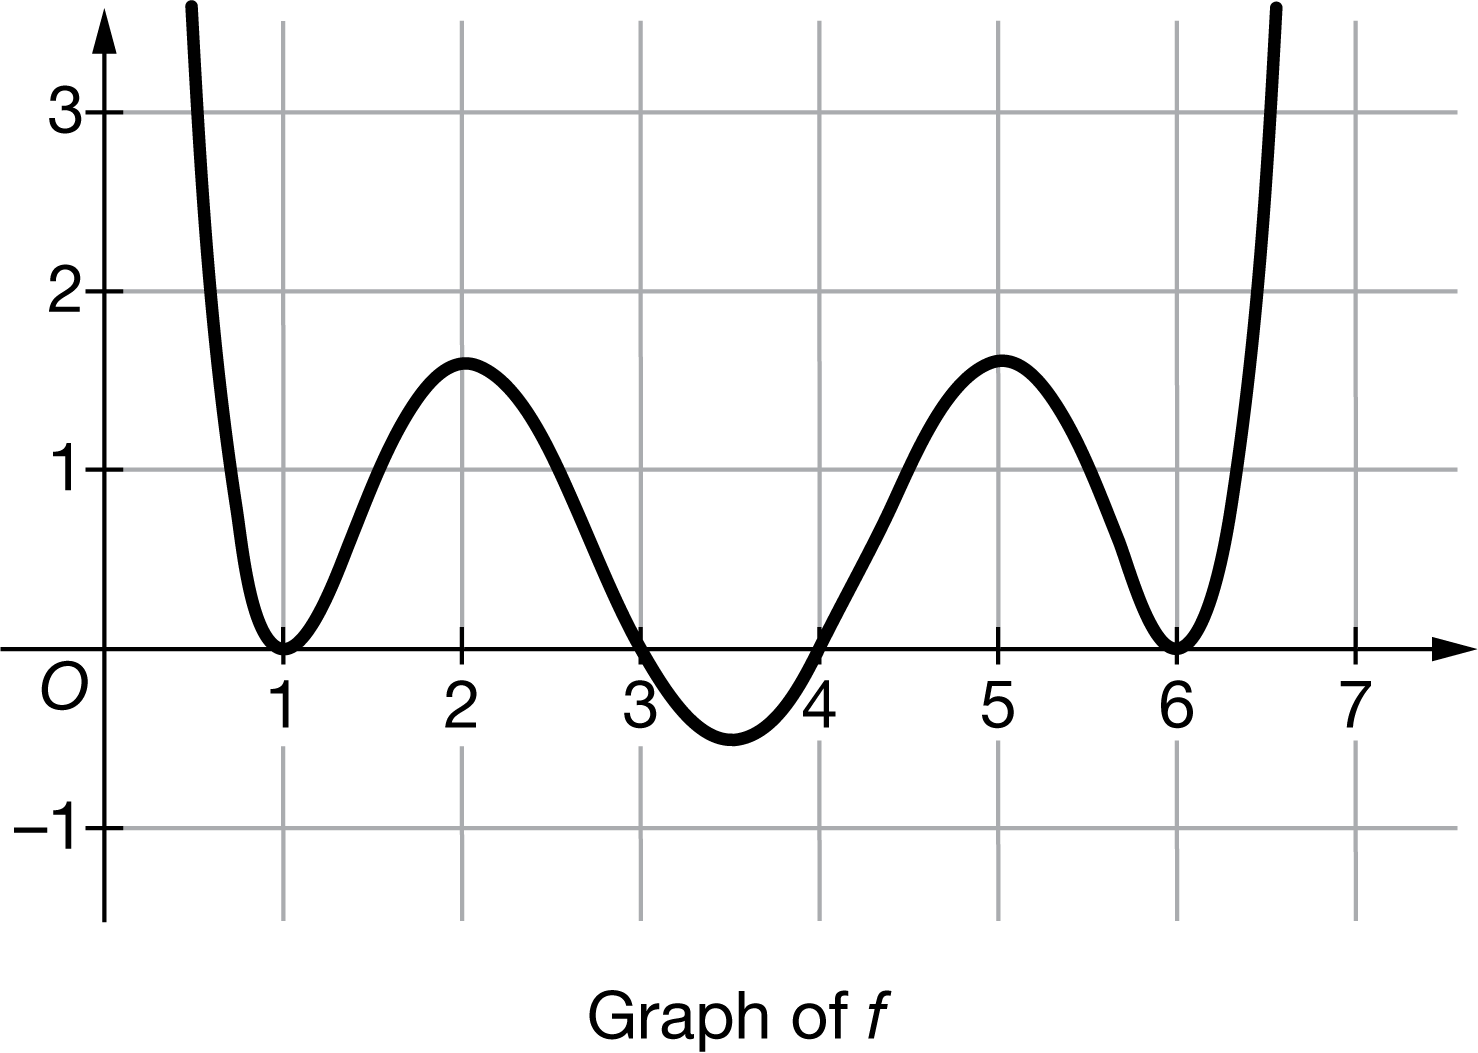
\includegraphics[width=2in]{original-21.png}
\end{center}
The graph of the function $f$ is shown above. Let $g$ be the function defined by $g(x)=\int_{1}^{x} f(t) \, dt$. At what values of $x$ in the interval $0.5<x<6.5$ does $g$ have a relative maximum?
\begin{enumerate}
    \item $g'(x)=f(x)$
    \item Relative maximum: $f$ changes from positive to negative.
\end{enumerate}
$$\boxed{\text{Relative maximum: } x=3}$$
\item The function $h$ is given by $h(x)=\int_{1}^{x} \ln(t\sin t +5) \, dt$ for $1 \leq x \leq 7$. On what intervals, if any, is $h$ decreasing?
\begin{enumerate}
    \item $h'(x)=\frac{d}{dx} \big(\int_{1}^{x} \ln(t\sin t +5) \big)=\ln(x \cdot \sin x +5)$
\end{enumerate}d
    $$\boxed{\text{When } x\in[4.323,5.461] \: h'(x)<0 \: \therefore \: f \text{ is decreasing.}}$$
\end{enumerate}
\section*{3.07}
\begin{enumerate}
    \item If $F$ and $f$ are differentiable functions such that $F(x)=\int_{0}^{x} f(t) \, dt$, and if $F(a)=-2$ and $F(b)=-2$ where $a<b$, which of the following must be true?
    $$\boxed{f(x)=0 \text{ for some } x \text{ such that } a<x<b.}$$
    \item 
    \begin{center}
        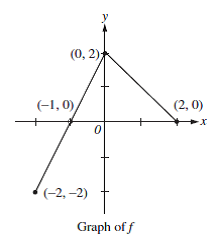
\includegraphics[width=2in]{original-22.png}
    \end{center}
    The graph of the function $f$ shown above consists of two line segments. If $g$ is the function defined by $g(x)=\int_{0}^{x}f(t)\,dt$, then $g(-1)=$
    $$g(-1)=\int_{0}^{-1}f(t)\,dt  = -\int_{-1}^{0}f(t)\,dt = -(0.5)(2)(1)=\boxed{-1}$$
    
    \item The function $f$ is given by $f(x)=\int_{1}^{x} \sqrt{t^3+2}\,dt$. What is the average rate of change of $f$ over the interval $[0,3]$?
    $$f_{\text{avg}}=\frac{f(3)-f(0)}{3-0}= \frac{\int_{1}^{3} f(x) \, dx - \int_{1}^{0} f(x) \, dx}{3} = \frac{\int_{1}^{3} f(x) \, dx + \int_{0}^{1} f(x) \, dx}{3} = \frac{\int_{0}^{3} f(x) \, dx}{3}$$
    
    $$ f_{\text{avg}}= \frac{\int_{0}^{3} f(x) \, dx}{3} \approx  \boxed{2.694}$$
    \item 
    \begin{center}
        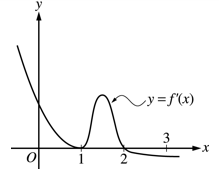
\includegraphics[width=2in]{original-23.png}
    \end{center}
    The graph of $f'$, the derivative of the function $f$, is shown above. If $f(0) = 0$, which of the following must be true?
    \begin{enumerate}[I.]
        \item $f(0) > f(1)$: \textit{False since the} $\int_{0}^{1} f'(x) \, dx > 0 \: \therefore f(1)>f(0).$
        \item $ f(2) > f(1)$ \textit{True since the} $\int_{1}^{2} f'(x) \, dx > 0 \: \therefore f(2)>f(1).$
        \item $f(1) > f(3)$ \textit{False since the} $\int_{0}^{1} f'(x) \, dx < \int_{0}^{3} f'(x) \, dx$
    \end{enumerate}
    $$\boxed{\text{II only}}$$
    \item 
    \begin{center}
        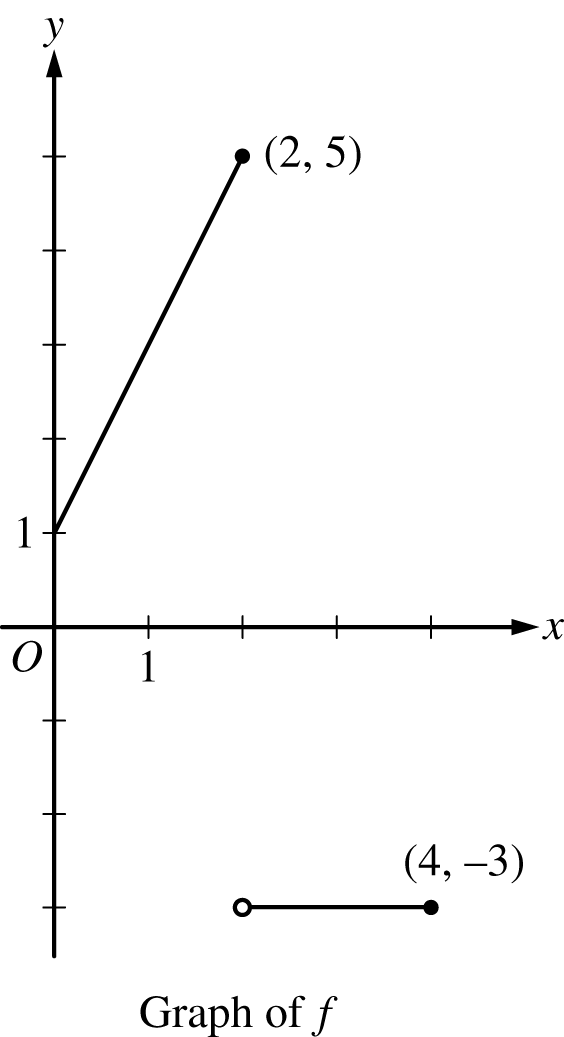
\includegraphics[width=2in]{original-24.png}
    \end{center}
    The graph of $f$ is shown above for $0 \leq x \leq 4$. What is the value of $\int_{0}^{4} f(x) \, dx$?
    $$\int_{0}^{4} f(x) \, dx = \int_{0}^{2} f(x) \, dx + \int_{2}^{4} f(x) \, dx$$
    $$\int_{0}^{4} f(x) \, dx =\frac{(1+5)\cdot 2}{2} + (2)(-3)= \boxed{0} $$
    \item Let $g$ be the function given by $g(x)=\int_{0}^{x} \sin(t^2) \, dt$ for $-1 \leq x \leq 3$. On which of the following intervals is $g$ decreasing?
    $$g'(x) = \frac{d}{dx} \biggr( \int_{0}^{x} \sin(t^2) \, dt \biggr) = \sin(x^2)$$
    $$\boxed{\text{When } x\in[1.772, 2.507] \: g'(x)<0 \: \therefore \: g \text{ is decreasing.}}$$
    \item Let $g$ be the function defined by $g(x)= \int_{-1}^{x}\frac{t^3-t^2-6t}{\sqrt{t^2+7}}\,dt $ On which of the following intervals is $g$ decreasing?
    $$g'(x)=\frac{d}{dx}\biggr(\int_{-1}^{x}\frac{t^3-t^2-6t}{\sqrt{t^2+7}}\,dt \biggr) =\frac{x^3-x^2-6x}{\sqrt{x^2+7}}=\frac{x(x-3)(x+2)}{\sqrt{x^2+7}}$$
    $$\boxed{\text{When } x\in[0, 3] \text{ and when } x\in(\infty,-2] \Longrightarrow\: g'(x)<0 \: \therefore \: g \text{ is decreasing.}}$$
    \newpage
    \item 
    \begin{center}
        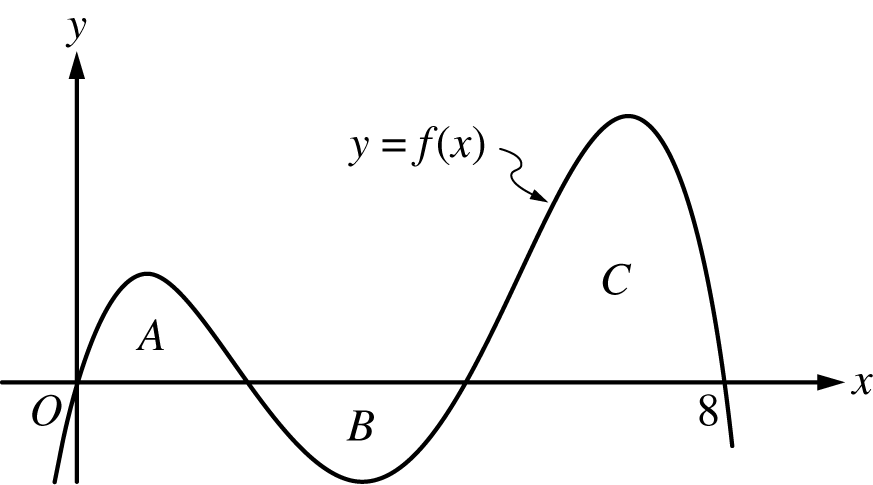
\includegraphics[width=3in]{original-25.png}
    \end{center}
    The regions $A$, $B$, and $C$ in the figure above are bounded by the graph of the function $f$ and the $x$-axis. The area of region $A$ is 14, the area of region $B$ is 16, and the area of region $C$ is 50. What is the average value of $f$ on the interval $[0,8]$?
    $$\int_{0}^{8} f(x) \, dx = 14-16+50=48$$
    $$f_{\text{avg}}= \frac{1}{8-0} \int_{0}^{8} f(x) \, dx = \boxed{6}$$
    
    \item $\frac{d}{dx} \biggr( \int_{0}^{x^3} \ln(t^2+1) \, dt \biggr)=$

$$\frac{d}{dx}\biggr( F(x^3)-F(0) \biggr)$$
 $$F'(x)=3x^2 \cdot F'(x^3)= \boxed{3x^2 \big( \ln(x^6+1) \big)}$$

    \item If $\int_{1}^{10} f(x) \,dx =4$ and $\int_{10}^{3} f(x) \, dx =7$ then $\int_{1}^{3} f(x) \, dx$
    $$\int_{1}^{10} f(x) \, dx = \int_{1}^{3} f(x) \,dx + \int_{3}^{10} f(x) \, dx$$
    $$\int_{1}^{10} f(x) \,dx - \int_{3}^{10} f(x) \,dx = \int_{1}^{3} \f(x) \,dx $$
    $$\int_{1}^{3} \f(x) \,dx = 4 - (-7) = \boxed{11}$$
    
\end{enumerate}
\section*{3.08}
\everymath{\displaystyle}
\begin{enumerate}
    \item Which of the following is a \underline{left Riemann sum} approximation of $\int_{1}^{7} (4\ln x+2) \, dx$ with $n$ subintervals of equal length?
    \begin{enumerate}
        \item $\Delta x = \frac{7-1}{n} = \frac{6}{n}$
        \item $x_k = a + \Delta x \cdot (k-1)  =  1 + \frac{6(k-1)}{n}$
    \end{enumerate}
   $$\Longrightarrow \boxed{ \lim_{n\to\infty} \sum_{k=1}^{n} \biggr[4\ln\bigg( 1 + \frac{6(k-1)}{n} \bigg) + 2 \biggr] \cdot \frac{6}{n}}$$
   
    \item Which of the following definite integrals are equal to $\lim_{n\to\infty} \sum_{k=1}^{n} \biggr(-2+\frac{8k}{n} \biggr)^3 \cdot \frac{8}{n}$
    \begin{enumerate}[I.]
        \item $\int_{-2}^{6} x^3 \, dx$: True assuming $\Delta x = \frac{8}{n}$ and $x_k = -2 + \frac{8k}{n}$
        \item $\int_{0}^{8} (-2+x)^3 \, dx$: True assuming $\Delta x = \frac{8}{n}$ and $x_k = \frac{8k}{n}$
        \item $8 \int_{0}^{1}(-2+8x)^3 \, dx$: True assuming $\Delta x = \frac{1}{n}$ and $x_k = \frac{k}{n}$
    \end{enumerate}
    $$\boxed{\text{I, II, and III}}$$
    
    \item Which of the following definite integrals are equal to $\lim_{n\to\infty} \sum_{k=1}^{n} \frac{12k}{n}\cos\biggr(1+\frac{4k}{n} \biggr) \cdot \frac{4}{n}$
    \begin{enumerate}
        \item $\Delta x = \frac{4}{n}$
        \item $x_k=\frac{4k}{n}$
    \end{enumerate}
    $$\Longrightarrow \boxed{\int_{0}^{4} 3x \cos(1+x) \, dx}$$
    \item  Which of the following is a \underline{left Riemann sum} approximation of $\int_{2}^{8} \cos(x^2) \, dx$ with $n$ subintervals of equal length?
\begin{enumerate}
        \item $\Delta x = \frac{8-2}{n} = \frac{6}{n}$
        \item $x_k = a + \Delta x \cdot (k-1)  =  2 + \frac{6(k-1)}{n}$
    \end{enumerate}
    $$\Longrightarrow \boxed{\lim_{n\to\infty} \sum_{k=1}^{n} \sin\biggr(2+\frac{6(k-1)}{n} \biggr)^2 \cdot \frac{6}{n}}$$
    \item Which of the following definite integrals are equal to $\lim_{n\to\infty} \sum_{k=1}^{n} \sin\biggr(-1+\frac{5k}{n} \biggr) \cdot \frac{5}{n}$
\begin{enumerate}[I.]
        \item $\int_{-1}^{4} \sin x \, dx$: True assuming $\Delta x = \frac{5}{n}$ and $x_k = -1 + \frac{5k}{n}$
        \item $\int_{0}^{5} \sin(-1+x) \, dx$: True assuming $\Delta x = \frac{5}{n}$ and $x_k = \frac{5k}{n}$
        \item $5 \int_{0}^{1} \sin(-1 +5x) \, dx$: True assuming $\Delta x = \frac{1}{n}$ and $x_k = \frac{k}{n}$
    \end{enumerate}
    $$\boxed{\text{I, II, and III}}$$
    
   \item Which of the following definite integrals are equal to $\lim_{n\to\infty} \sum_{k=1}^{n} \frac{10k}{n}\biggr(\sqrt{1+\frac{5k}{n}} \biggr) \cdot \frac{5}{n}$
$$\Longrightarrow \boxed{\int_{0}^{5} 2x\sqrt{1+x} \, dx}$$
   
   \item Which of the following limits is equal to $\int_{2}^{5} x^2 \, dx$
   \begin{enumerate}
        \item $\Delta x = \frac{5-2}{n} = \frac{5}{n}$
        \item $x_k = a + \Delta x \cdot k  =  2 + \frac{5k}{n}$
    \end{enumerate}
    $$\Longrightarrow \boxed{\lim_{n\to\infty} \sum_{k=1}^{n} \biggr(2+ \frac{3k}{n} \biggr)^2 \cdot \frac{3}{n}}$$
    \item 
    \begin{center}
        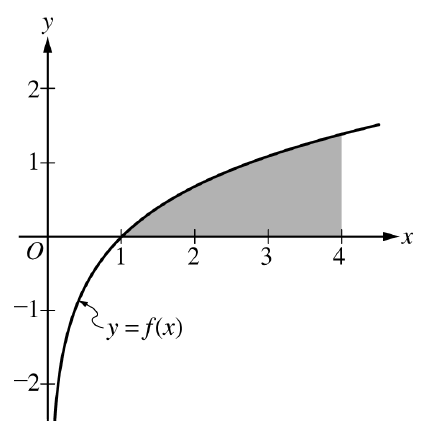
\includegraphics[width=2in]{original-26.png}
    \end{center}
    The function $f$ is given by $f(x) = \ln x$. The graph of $f$ is shown above. Which of the following limits is equal to the area of the shaded region?
    $$\Longrightarrow \int_{1}^{4} f(x) \, dx = \int_{1}^{4} \ln(x) \, dx  $$
    \begin{enumerate}
        \item $\Delta x = \frac{4-2}{n} = \frac{3}{n}$
        \item $x_k = a + \Delta x \cdot k  =  1 + \frac{3k}{n}$
    \end{enumerate}
      $$\Longrightarrow \boxed{\lim_{n\to\infty} \sum_{k=1}^{n} \ln \biggr(1+ \frac{3k}{n}\biggr) \cdot \frac{3}{n}}$$
\end{enumerate}
\end{document}